\documentclass[11pt,a4paper,openany]{book}
\usepackage[a4paper,top=24mm,bottom=23mm,left=24mm,right=24mm,headheight=15pt]{geometry}
\usepackage[T1]{fontenc}
\usepackage{lmodern}
\usepackage{microtype}
\usepackage{parskip}
\usepackage{setspace}
\usepackage{xcolor}
\usepackage{tikz}
\usetikzlibrary{arrows.meta,positioning,shapes.geometric}
\usepackage{booktabs}
\usepackage{tabularx}
\usepackage{longtable}
\usepackage{enumitem}
\usepackage{listings}
\usepackage{tcolorbox}
\usepackage{titlesec}
\usepackage{fancyhdr}
\usepackage{hyperref}
\usepackage{bookmark}

\definecolor{ink}{HTML}{17324D}
\definecolor{teal}{HTML}{087F8C}
\definecolor{tealsoft}{HTML}{E8F5F5}
\definecolor{gold}{HTML}{B97800}
\definecolor{goldsoft}{HTML}{FFF5D8}
\definecolor{red}{HTML}{B42318}
\definecolor{redsoft}{HTML}{FFF0EE}
\definecolor{codebg}{HTML}{F4F7F8}
\definecolor{codeborder}{HTML}{D5E1E5}
\definecolor{muted}{HTML}{5B6B78}
\definecolor{linegray}{HTML}{D7E0E4}

\hypersetup{colorlinks=true,linkcolor=teal,urlcolor=teal,pdftitle={Production Foundations Learning Journey},pdfauthor={Codex}}
\setstretch{1.16}
\setlength{\parindent}{0pt}
\setlength{\parskip}{6pt}
\setlength{\emergencystretch}{3em}
\setlist[itemize]{leftmargin=*,itemsep=2pt,topsep=3pt}
\setlist[enumerate]{leftmargin=*,itemsep=3pt,topsep=3pt}
\titleformat{\chapter}[display]{\normalfont\bfseries\color{ink}}{\filleft\Large\chaptertitlename\ \thechapter}{8pt}{\Huge}
\titlespacing*{\chapter}{0pt}{-10pt}{24pt}
\titleformat{\section}{\Large\bfseries\color{teal}}{\thesection}{0.65em}{}
\titleformat{\subsection}{\large\bfseries\color{ink}}{\thesubsection}{0.6em}{}
\titlespacing*{\section}{0pt}{22pt}{8pt}
\titlespacing*{\subsection}{0pt}{15pt}{5pt}
\pagestyle{fancy}
\fancyhf{}
\fancyhead[LE,RO]{\small\color{muted}Production Foundations}
\fancyhead[RE,LO]{\small\color{muted}\nouppercase{\leftmark}}
\fancyfoot[C]{\small\color{muted}\thepage}
\renewcommand{\headrulewidth}{0.3pt}
\lstdefinestyle{shell}{basicstyle=\ttfamily\small,backgroundcolor=\color{codebg},frame=single,rulecolor=\color{codeborder},framerule=0.4pt,breaklines=true,breakatwhitespace=false,columns=fullflexible,keepspaces=true,showstringspaces=false,aboveskip=8pt,belowskip=8pt,xleftmargin=5pt,xrightmargin=5pt}
\lstset{style=shell}
\newtcolorbox{mentalbox}[1]{colback=tealsoft,colframe=teal,boxrule=0.7pt,arc=2pt,left=8pt,right=8pt,top=7pt,bottom=7pt,title={\textbf{#1}},fonttitle=\color{teal}}
\newtcolorbox{safetybox}[1]{colback=redsoft,colframe=red,boxrule=0.7pt,arc=2pt,left=8pt,right=8pt,top=7pt,bottom=7pt,title={\textbf{Safety: #1}},fonttitle=\color{red}}
\newtcolorbox{trybox}[1]{colback=goldsoft,colframe=gold,boxrule=0.7pt,arc=2pt,left=8pt,right=8pt,top=7pt,bottom=7pt,title={\textbf{Try it: #1}},fonttitle=\color{gold}}
\newtcolorbox{explainbox}[1]{colback=white,colframe=linegray,boxrule=0.6pt,arc=2pt,left=8pt,right=8pt,top=7pt,bottom=7pt,title={\textbf{Read the command: #1}},fonttitle=\color{ink}}
\newcommand{\command}[1]{\texttt{\small\detokenize{#1}}}
\newcommand{\lesson}[1]{\begin{mentalbox}{Where you are in the journey}#1\end{mentalbox}}
\newcommand{\checkpoint}[1]{\begin{mentalbox}{Checkpoint}\textbf{#1}\end{mentalbox}}
\begin{document}
\begin{titlepage}
\thispagestyle{empty}
\vspace*{18mm}
{\color{teal}\rule{\textwidth}{2pt}}\\[15mm]
{\Huge\bfseries\color{ink}Production Foundations\\[4pt]Learning Journey}\par
\vspace{9mm}
{\Large\color{muted}Linux, curl, command-line tools, VMs, SSH, cron, Docker, Nginx, and the habits that connect them}\par
\vfill
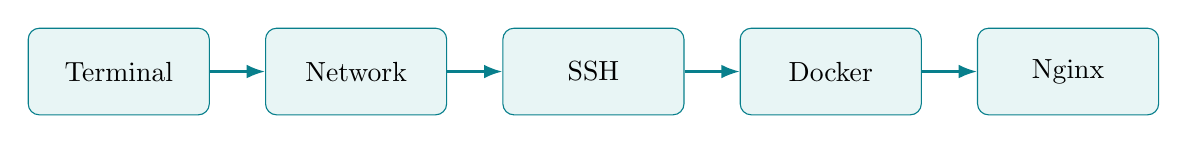
\begin{tikzpicture}[node distance=7mm,>=Latex]
\node[draw=teal,fill=tealsoft,rounded corners,minimum width=23mm,minimum height=11mm,align=center] (a) {Terminal};
\node[draw=teal,fill=tealsoft,rounded corners,minimum width=23mm,minimum height=11mm,align=center,right=of a] (b) {Network};
\node[draw=teal,fill=tealsoft,rounded corners,minimum width=23mm,minimum height=11mm,align=center,right=of b] (c) {SSH};
\node[draw=teal,fill=tealsoft,rounded corners,minimum width=23mm,minimum height=11mm,align=center,right=of c] (d) {Docker};
\node[draw=teal,fill=tealsoft,rounded corners,minimum width=23mm,minimum height=11mm,align=center,right=of d] (e) {Nginx};
\draw[->,thick,teal] (a)--(b); \draw[->,thick,teal] (b)--(c); \draw[->,thick,teal] (c)--(d); \draw[->,thick,teal] (d)--(e);
\end{tikzpicture}
\vfill
\parbox{0.84\textwidth}{\centering\large A hands-on course for a beginner using one disposable Ubuntu VM on Windows}\par
\vspace{5mm}
{\color{muted}July 2026}\par
\end{titlepage}
\frontmatter
\chapter*{How to use this book}
\addcontentsline{toc}{chapter}{How to use this book}
This is a journey, not a dictionary. Each chapter gives you a small mental model, one safe command at a time, and a checkpoint that proves what you understood. Keep an Ubuntu virtual machine open while you read. Make a snapshot before any lesson that changes networking, SSH, firewall rules, or services.
The examples use Linux syntax. Your output will vary with your username, IP address, package versions, and current time; learn to recognize the shape of the result instead of memorizing one exact line.
\begin{mentalbox}{The repeating lesson pattern}
Every practical example follows the same rhythm: problem, command, explanation, expected output, interpretation, common mistake, and a small exercise. If a command feels mysterious, stop after the explanation and run it again with one option removed.
\end{mentalbox}
\chapter*{The route through the course}
\addcontentsline{toc}{chapter}{The route through the course}
\begin{enumerate}
\item Create a safe Linux lab.
\item Learn the terminal and use curl to make your first request.
\item Create, find, edit, transform, and move files.
\item Inspect the machine and understand permissions.
\item Diagnose a network from the URL outward.
\item Connect to another machine with SSH.
\item Schedule and supervise recurring work.
\item Package an application with Docker.
\item Put Nginx in front of it and deploy it carefully.
\item Finish by operating a small service and explaining every layer.
\end{enumerate}
\tableofcontents
\mainmatter
\chapter{Your first safe Linux lab}
\lesson{Before learning commands, you need a place where mistakes are cheap. A virtual machine is a computer made of files, running inside your Windows computer.}
\section{What the terminal actually is}
The graphical desktop is one way to ask the operating system for work. The terminal is another. You type a command; a shell reads it, finds a program, supplies arguments, and displays output. Bash is one shell; Zsh and PowerShell are other shells with different syntax.
When you see a prompt such as \command{alice@ubuntu:~\$}, the pieces are clues: \command{alice} is the user, \command{ubuntu} is the machine, the tilde means the home directory, and the dollar sign says this is an ordinary user prompt. A prompt ending in a hash sign usually means a privileged root shell.
\begin{lstlisting}[language=bash]
whoami
hostname
printf 'The shell is running a command.\n'
\end{lstlisting}
\begin{explainbox}{three tiny commands}
\command{whoami} asks which user owns this shell. \command{hostname} prints the machine name, useful when several terminals look similar. \command{printf} writes exactly the text you provide; the backslash-n escape requests a new line. None of these commands changes files.
\end{explainbox}
\section{Create the Ubuntu VM}
Install VirtualBox, download an Ubuntu LTS desktop ISO, and create a VM with roughly two virtual CPUs, 4--8 GB of RAM, and a dynamically allocated disk of at least 25 GB. Exact values depend on your laptop. Start with NAT networking. NAT lets the VM reach the internet while keeping inbound connections from the internet out of the VM by default.
During installation, create a normal user with a strong passphrase. Use \command{sudo} only when a task genuinely needs administrator rights. That separation is part of the lesson: a command that can rewrite the whole machine should not be the default identity.
\begin{mentalbox}{Snapshot before experiments}
Take a VM snapshot named \emph{fresh-install} now. Take another named \emph{after-ssh} before changing SSH, firewall, or network settings. A snapshot is not a backup, but it is a fast way to return to a known practice state.
\end{mentalbox}
\section{First checkpoint}
\begin{lstlisting}[language=bash]
mkdir -p ~/journey/{notes,downloads,lab}
ls -la ~/journey
\end{lstlisting}
The \command{-p} option allows \command{mkdir} to create missing parent directories. Braces are expanded by Bash into three names before \command{mkdir} runs. \command{ls -la} means ``list, including hidden entries, in a detailed format.''
\checkpoint{You can identify the user, identify the VM, create a course workspace, and explain why the VM is a safer place to practise privileged commands.}
\chapter{curl: see a real request}
\lesson{curl is the first tool in the journey because it makes the invisible visible. You can ask a server for a page, inspect headers, save a response, and turn the result into a test.}
\section{The smallest useful request}
\begin{lstlisting}[language=bash]
curl https://example.com
\end{lstlisting}
\begin{explainbox}{the URL and default output}
\command{curl} is the program. The URL has a scheme (\command{https}), a host (\command{example.com}), and an optional path. With no output option, curl writes the response body to the terminal. It transfers bytes; it does not open a graphical browser.
\end{explainbox}
Try a response that is easier to read:
\begin{lstlisting}[language=bash]
curl -i https://example.com
\end{lstlisting}
The short option \command{-i} means ``include response headers.'' The first line is the HTTP status, followed by headers such as content type, then a blank line, then the body.
\section{Read the flags one at a time}
\begin{lstlisting}[language=bash]
curl -I https://example.com
curl -v https://example.com
curl -sS https://example.com
curl -fsS https://example.com/health
\end{lstlisting}
\begin{itemize}
\item \command{-I} sends a HEAD request and asks for headers without the normal body. Some servers handle HEAD differently.
\item \command{-v} enables verbose diagnostics: DNS, connection, TLS negotiation, request headers, and response headers.
\item \command{-sS} hides progress output but still shows errors, keeping scripts readable.
\item \command{-f} returns a failure exit code for HTTP 400 and later. The transfer may have worked while the application request failed.
\end{itemize}
\begin{safetybox}{do not normalise -k}
\command{-k} disables TLS certificate verification. Use it only for a deliberately local test with a self-signed certificate; fix trust failures in production.
\end{safetybox}
\section{Save, inspect, and test}
\begin{lstlisting}[language=bash]
curl --fail --location --output ~/journey/downloads/page.html \
  https://example.com
wc -c ~/journey/downloads/page.html
head -n 5 ~/journey/downloads/page.html
\end{lstlisting}
\begin{explainbox}{download options}
\command{--fail} makes HTTP errors visible to automation. \command{--location} follows redirects. \command{--output path} writes the body to a named file. The trailing backslash joins the next line into one command.
\end{explainbox}
\begin{lstlisting}[language=bash]
curl --fail-with-body --silent --show-error \
  --max-time 10 --retry 3 https://example.com/health
echo "curl exit code: $?"
\end{lstlisting}
The question mark expression reads the previous command's exit status. Zero means curl completed successfully. A non-zero value tells a script to take a failure path. The timeout and retries do not make a broken application healthy.
\section{JSON APIs with jq}
\begin{lstlisting}[language=bash]
curl --fail --silent --show-error \
  https://api.github.com/repos/curl/curl \
  | jq '{name, stars: .stargazers_count, language}'
\end{lstlisting}
The pipe sends curl's output to \command{jq}. The jq expression constructs a smaller object from named JSON fields. This is safer than grepping JSON because jq understands data types and nesting.
\begin{trybox}{curl practice}
Request \url{https://httpbin.org/status/404} with and without \command{-f}. Observe the body, the terminal error, and \command{\$?}. Then request \url{https://httpbin.org/redirect/1} with and without \command{--location}. Explain why the results differ.
\end{trybox}
\checkpoint{You can separate a URL, request, response headers, body, and exit status. You can write a curl health check that fails loudly without leaking progress noise into logs.}
\chapter{The everyday command-line toolbelt}
\lesson{The shell becomes powerful when small programs cooperate. Learn each tool as a narrow instrument, then combine them with pipes and redirection.}
\section{Files, paths, and safe movement}
\begin{lstlisting}[language=bash]
cd ~/journey/lab
printf 'first line\nsecond line\n' > notes.txt
cp notes.txt notes-copy.txt
mv notes-copy.txt archive.txt
ls -l
\end{lstlisting}
The greater-than sign redirects output into a file and replaces an existing file. Two greater-than signs append instead. \command{cp} creates a second file; \command{mv} changes its name or location. The \command{-l} form of \command{ls} shows mode bits, owner, size, and modification time.
\begin{safetybox}{redirection and rm}
Before using \command{>} or \command{rm}, print the path with \command{pwd} and \command{ls}. Practise destructive commands only in a disposable folder.
\end{safetybox}
\section{Search and transform text}
\begin{lstlisting}[language=bash]
rg --line-number 'second' ~/journey/lab
find ~/journey -type f -name '*.txt'
cat notes.txt | tr 'a-z' 'A-Z'
sort notes.txt | uniq -c
\end{lstlisting}
\command{rg} searches file contents and shows matching line numbers. \command{find} searches the filesystem using predicates. \command{tr} translates characters. \command{sort} orders lines so \command{uniq -c} can count adjacent duplicates.
\section{Nano and Vim}
Nano is a modeless editor. Open a file with \command{nano notes.txt}; type normally; press \command{Ctrl+O} to write and \command{Ctrl+X} to exit. The caret symbol in Nano's help means the Control key.
Vim is modal. Start with \command{vim notes.txt}. Press \command{i} to insert, Escape for Normal mode, type \command{:w} and Enter to save, and \command{:q} and Enter to quit. \command{:wq} saves and quits; \command{:q!} quits without saving.
\begin{mentalbox}{Why Vim feels unusual}
Vim separates navigation from insertion. Learn insert, escape, save, quit, search, and undo first; postpone advanced commands.
\end{mentalbox}
\section{FFmpeg and ffprobe}
\begin{lstlisting}[language=bash]
ffprobe -hide_banner recording.mp4
ffmpeg -i recording.mp4 -vn -c:a copy audio.m4a
ffmpeg -i recording.mp4 -vf scale=1280:-2 -c:v libx264 -crf 23 preview.mp4
\end{lstlisting}
\command{ffprobe} reports streams, codecs, dimensions, duration, and metadata. \command{-i} names the input, \command{-vn} removes video, and \command{-c:a copy} copies audio without re-encoding. The scale filter preserves aspect ratio; CRF controls H.264 quality. Re-encoding takes time and can reduce quality.
\section{A small pipeline}
\begin{lstlisting}[language=bash]
curl --fail --silent https://example.com/robots.txt \
  | tee ~/journey/notes/robots.txt \
  | wc -l
\end{lstlisting}
\command{tee} writes the stream to a file and also passes it onward. The final \command{wc -l} counts lines. Observe each boundary before deciding whether the next tool received what you intended.
\checkpoint{You can edit a file in Nano, save and quit in Vim, search with rg, inspect media with ffprobe, and explain where a pipe sends data.}

\chapter{Users, permissions, processes, and logs}
\lesson{A production machine is shared by people and programs. Linux permissions, process ownership, and logs are the language that prevents one task from silently damaging another.}
\section{Read permission bits}
\begin{lstlisting}[language=bash]
ls -l ~/journey/lab/notes.txt
chmod u+x ~/journey/lab/notes.txt
stat ~/journey/lab/notes.txt
\end{lstlisting}
The first character of the long listing describes the type. The next three groups describe permissions for the owner, group, and everyone else. \command{r} reads, \command{w} writes, and \command{x} executes or enters a directory. \command{chmod u+x} adds execute permission for the user without disturbing other bits.
\section{sudo and packages}
\begin{lstlisting}[language=bash]
sudo apt update
apt list --upgradable
sudo apt install jq tree
command -v jq
\end{lstlisting}
\command{sudo} asks for temporary administrative authority. \command{apt update} refreshes package metadata; it does not upgrade packages. \command{apt install} resolves and installs the named packages. \command{command -v} shows which executable the shell will run.
\section{Processes and signals}
\begin{lstlisting}[language=bash]
sleep 120 &
jobs -l
ps -ef | rg '[s]leep 120'
kill PID
\end{lstlisting}
The ampersand starts a background command. \command{jobs -l} shows shell-managed jobs and their process IDs. Replace \command{PID} with the actual number. \command{kill} sends SIGTERM by default, asking a cooperative process to stop; SIGKILL is a last resort.
\section{Logs are evidence}
\begin{lstlisting}[language=bash]
journalctl -b --no-pager | tail -n 30
df -h
free -h
\end{lstlisting}
\command{journalctl -b} limits the system journal to the current boot. \command{--no-pager} prints directly. \command{df -h} reports filesystem capacity; \command{free -h} reports memory. Inspect the machine before changing application code.
\checkpoint{You can explain who owns a file, what a process is doing, and which command shows logs, disk, or memory evidence.}

\chapter{Networking from the URL outward}
\lesson{When a request fails, walk from the name to the wire: URL parsing, DNS, route, socket, TLS, HTTP, and application data. Each layer has different evidence.}
\section{Name, address, route, socket}
\begin{lstlisting}[language=bash]
ip addr
ip route
getent hosts example.com
ss -tulpn
\end{lstlisting}
\command{ip addr} lists interfaces and addresses. \command{ip route} shows where packets go. \command{getent hosts} asks the system resolver for a name. \command{ss -tulpn} lists listening TCP and UDP sockets.
\section{A diagnostic sequence}
\begin{lstlisting}[language=bash]
ping -c 3 1.1.1.1
dig example.com
nc -vz example.com 443
curl -vI https://example.com
\end{lstlisting}
Ping tests one kind of reachability and may be blocked even when HTTPS works. \command{dig} shows DNS answers and timing. \command{nc -vz} attempts a TCP connection without transferring application data. curl then shows the TLS and HTTP layers.
\section{VM networking and UFW}
NAT is convenient for outbound access. Bridged mode gives the VM an address on the same LAN as Windows when another device must reach a service in the VM. Before switching modes, record the current address and take a snapshot.
\begin{lstlisting}[language=bash]
sudo ufw status verbose
sudo ufw allow OpenSSH
sudo ufw enable
\end{lstlisting}
\begin{safetybox}{firewall lockout}
Never enable a firewall on a remote machine before allowing your management path. Test SSH in a second terminal before closing the first session.
\end{safetybox}
\checkpoint{You can tell whether a failure is probably DNS, a route, a closed port, TLS, HTTP, or an application response.}

\chapter{SSH: operate another machine}
\lesson{SSH turns a network connection into a remote terminal. It is the bridge from your practice VM to a cloud server, another VM, a Git host, or a production machine.}
\section{Keys, locks, and fingerprints}
\begin{lstlisting}[language=bash]
ssh-keygen -t ed25519 -C "journey@example.com"
cat ~/.ssh/id_ed25519.pub
chmod 700 ~/.ssh
chmod 600 ~/.ssh/id_ed25519
\end{lstlisting}
The public key is safe to place on a server; the private key is secret. Ed25519 is a modern compact key type. The passphrase protects the private key if the file is copied. The directory and file modes prevent other local users from reading key material.
\section{Connect and verify}
\begin{lstlisting}[language=bash]
ssh ubuntu@192.168.56.20
ssh -o ConnectTimeout=5 ubuntu@192.168.56.20 'hostname; uptime'
\end{lstlisting}
The first command opens an interactive shell. The second runs a remote command and returns to the local shell. On first connection, SSH shows the server fingerprint. Verify it through a trusted channel before accepting it.
\section{Copy files and use an agent}
\begin{lstlisting}[language=bash]
scp notes.txt ubuntu@192.168.56.20:~/journey/
rsync -av --dry-run ~/journey/ ubuntu@192.168.56.20:~/journey/
ssh-add ~/.ssh/id_ed25519
\end{lstlisting}
\command{scp} performs a simple copy over SSH. \command{rsync -av --dry-run} previews a recursive archive-mode synchronization without changing the destination. Remove \command{--dry-run} only after the file list is correct. \command{ssh-add} loads a private key into the agent.
\begin{mentalbox}{SSH checklist}
Use keys with passphrases, verify fingerprints, restrict permissions, use a host alias in \textasciitilde/.ssh/config, and keep a second recovery session while changing SSH settings.
\end{mentalbox}
\checkpoint{You can distinguish a public key from a private key, make a safe first connection, and preview a file transfer.}

\chapter{Services, cron, and reliable schedules}
\lesson{A command you ran once is not yet a service. Reliability comes from a clear owner, a schedule, logs, timeouts, locking, and an alert when the expected result is missing.}
\section{A systemd service}
\begin{lstlisting}[language=bash]
systemctl status ssh --no-pager
systemctl list-units --type=service --state=running
journalctl -u ssh -b --no-pager
\end{lstlisting}
\command{systemctl status} shows state, recent logs, the unit file, and the main process. \command{list-units} provides an inventory. \command{journalctl -u ssh} filters evidence to one service.
\section{Cron basics}
Cron fields are minute, hour, day of month, month, and day of week. A schedule is only one part of a job; use absolute paths, explicit environment variables, a log destination, a timeout, and overlap protection.
\begin{lstlisting}[language=bash]
crontab -l
crontab -e
\end{lstlisting}
For a safe practice job, add:
\begin{lstlisting}[language=bash]
*/5 * * * * /usr/bin/date >> /home/ubuntu/journey/notes/cron.log 2>&1
\end{lstlisting}
The first field means every five minutes. The other four asterisks mean every hour, day, month, and weekday. The absolute path avoids relying on cron's smaller PATH. \command{2\&1} combines standard error with standard output.
\begin{mentalbox}{What people mean by a cron manager}
This phrase can mean a local crontab editor, a host dashboard that creates schedules, a heartbeat monitor, or a workflow scheduler such as Airflow. The manager does not remove the need to define idempotency, retries, logs, ownership, and alerting.
\end{mentalbox}
\section{systemd timers and overlap protection}
Systemd timers can express calendar schedules, persist missed runs, and connect naturally to service logs. For a job that must not overlap, use a lock:
\begin{lstlisting}[language=bash]
flock -n /tmp/journey.lock \
  /usr/bin/curl --fail --silent --show-error \
  --max-time 10 https://example.com/health
\end{lstlisting}
\command{flock -n} exits immediately if another copy owns the lock. A production job should also record success and send a heartbeat to a monitor.
\begin{trybox}{schedule practice}
Create a cron job that appends the date to a disposable file, wait for two runs, then inspect it with \command{tail}. Move the same task to a systemd timer and compare the logs.
\end{trybox}
\checkpoint{You can explain cron's five fields, the difference between cron and systemd timers, and why a scheduled job needs logging and locking.}

\chapter{Docker: package the application}
\lesson{Docker gives a process a repeatable filesystem, dependencies, environment, and network boundary. It does not replace Linux knowledge; it makes that knowledge easier to reproduce.}
\section{Image, container, volume, network}
An image is a read-only template. A container is a running process created from that template. A volume stores data outside the container's writable layer. A Docker network gives containers a private way to find each other by service name.
\begin{lstlisting}[language=bash]
docker version
docker run --rm hello-world
docker ps -a
\end{lstlisting}
\command{docker version} checks client and daemon. \command{docker run} creates and starts a container; \command{--rm} removes it after exit. \command{docker ps -a} lists running and stopped containers.
\section{A Dockerfile, line by line}
\begin{lstlisting}
FROM python:3.12-slim
WORKDIR /app
COPY requirements.txt .
RUN pip install --no-cache-dir -r requirements.txt
COPY app.py .
EXPOSE 8000
CMD ["python", "app.py"]
\end{lstlisting}
\command{FROM} chooses the base filesystem. \command{WORKDIR} sets the process directory. \command{COPY} adds files. \command{RUN} executes during build, while \command{CMD} supplies the default runtime command. \command{EXPOSE} documents a port; it does not publish it.
\begin{lstlisting}[language=bash]
docker build -t journey-api:dev .
docker run --rm -p 8000:8000 journey-api:dev
curl --fail http://127.0.0.1:8000/health
\end{lstlisting}
The final dot is the build context. \command{-t} gives the image a name and tag. \command{-p 8000:8000} maps host port 8000 to container port 8000. The application must listen on the container network interface, not only on 127.0.0.1 inside the container.
\section{Compose and persistence}
Compose describes related services in one file, including ports, environment, dependencies, and volumes. Use \command{docker compose up --build} to build and start, \command{docker compose logs -f} to follow logs, and \command{docker compose down} to stop. Named volumes survive container replacement; they are not backups.
\begin{mentalbox}{Container debugging order}
Check \command{docker ps}, then \command{docker logs}, then the published port, then the process's bind address, then the dependency network. Change one variable at a time.
\end{mentalbox}
\checkpoint{You can distinguish an image, container, volume, and network, and you know what each Dockerfile instruction does.}

\chapter{Nginx, HTTPS, and the edge}
\lesson{Nginx is the public-facing door. It can serve static files, terminate TLS, choose an upstream application, and provide a stable place for logs and headers.}
\section{Reverse proxy mental model}
\begin{center}
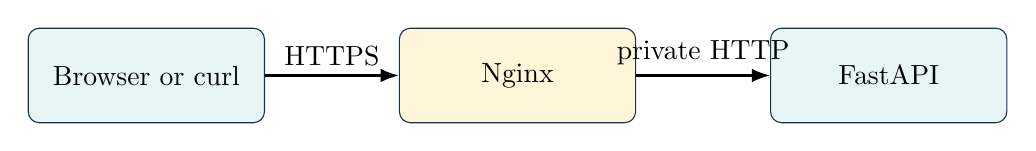
\begin{tikzpicture}[node distance=17mm,>=Latex]
\node[draw=ink,fill=tealsoft,rounded corners,minimum width=30mm,minimum height=12mm] (client) {Browser or curl};
\node[draw=ink,fill=goldsoft,rounded corners,minimum width=30mm,minimum height=12mm,right=of client] (nginx) {Nginx};
\node[draw=ink,fill=tealsoft,rounded corners,minimum width=30mm,minimum height=12mm,right=of nginx] (app) {FastAPI};
\draw[->,thick] (client)--node[above]{HTTPS}(nginx);
\draw[->,thick] (nginx)--node[above]{private HTTP}(app);
\end{tikzpicture}
\end{center}
The public client sees one stable hostname. Nginx handles certificates and forwards an internal request to the application. The application does not need to be directly reachable from the internet.
\section{A minimal server block}
\begin{lstlisting}
server {
    listen 80;
    server_name example.com;
    location / {
        proxy_pass http://127.0.0.1:8000;
        proxy_set_header Host $host;
        proxy_set_header X-Forwarded-For $proxy_add_x_forwarded_for;
    }
}
\end{lstlisting}
\command{listen} chooses the public port. \command{server_name} selects the hostname. \command{location /} matches every path. \command{proxy_pass} forwards the request. Forwarded headers preserve the original host and client chain.
\begin{lstlisting}[language=bash]
sudo nginx -t
sudo systemctl reload nginx
curl -I http://example.com
\end{lstlisting}
Always test configuration before reloading. A reload is usually less disruptive than a restart. Add HTTPS only after DNS, port 80, and the application path work predictably.
\section{TLS and secrets}
TLS provides encryption and server identity. Certificate renewal is an operational process, not a one-time checkbox. Keep private keys outside Git, inject application secrets through a controlled mechanism, and check which users and processes can read them.
\checkpoint{You can describe the request path through Nginx, test configuration before reload, and explain why TLS verification and secret storage matter.}

\chapter{Git, deployment, and observability}
\lesson{Deployment is a controlled change. Git tells you what changed, a health check tells you whether the service works, and logs and metrics tell you why it does not.}
\section{A small Git loop}
\begin{lstlisting}[language=bash]
git status
git diff
git add app.py
git commit -m "Add health endpoint"
git log --oneline -5
\end{lstlisting}
\command{git status} is the inventory. \command{git diff} is the evidence. \command{git add} selects exact files. The commit records a recoverable change. Read the diff before staging; Git does not understand whether a secret is safe to commit.
\section{Health, readiness, and logs}
A liveness check asks ``is the process alive?'' A readiness check asks ``can it serve useful traffic?'' Use curl with a timeout and failure handling; record response time and status.
\begin{lstlisting}[language=bash]
curl --fail --silent --show-error --max-time 5 \
  --write-out '\nstatus=%{http_code} time=%{time_total}s\n' \
  http://127.0.0.1:8000/health
\end{lstlisting}
The \command{--write-out} template prints metadata after the body. A status of 200 is useful evidence, while timing helps reveal a slow dependency. Keep secrets out of command lines because shell history and process listings can expose them.
\section{Backups and rollback}
A backup is only real after a restore test. A rollback is only real after you know which image, commit, or package set was previously healthy. Write the procedure before the incident and practise it on the VM.

\chapter{Capstone: a small service from laptop to production shape}
\lesson{This final project joins the layers. You will build a tiny API, test it with curl, package it with Docker, schedule a maintenance check, and expose it through Nginx.}
\section{Build the application}
Create a disposable folder and a minimal FastAPI service. Run it locally first, then request \command{/health} with curl. Record the process ID, listening address, and response status. The application is intentionally small so the operational steps remain visible.
\section{Containerise and compose}
Build the image, run it on a private port, and check logs. Add a Compose file with an application service and a named volume only if the application needs persistent data. Use service names for internal discovery, not hard-coded container IP addresses.
\section{Put Nginx at the edge}
Configure a server block, test it, reload it, and verify the complete path: client to Nginx, Nginx to the container, application response, and logs at both layers. Only then add DNS and TLS.
\section{Schedule an operational task}
Create either a cron entry or systemd timer that calls the health endpoint with curl, uses a timeout, writes a timestamped log, and sends a heartbeat. Add a lock so two copies cannot overlap. Stop the application deliberately and observe the failure evidence.
\section{Fault-injection checklist}
\begin{enumerate}
\item Use the wrong hostname and identify the DNS symptom.
\item Stop the container and identify the connection symptom.
\item Break the Nginx upstream port and read both logs.
\item Fill a disposable log file and identify the disk symptom.
\item Run the scheduled check with a missing environment variable and fix its non-interactive environment.
\end{enumerate}
\checkpoint{You can explain the request path, process owner, network boundary, scheduler, logs, and rollback point for your service.}

+
\chapter{Worked examples: command to evidence}
\lesson{The fastest way to become comfortable is to read a command and its result as one story. These scenarios deliberately show the reasoning between typing and deciding.}
\section{Example: a health check that fails correctly}
Suppose an application exposes \command{/health}. Start with a readable interactive check:
\begin{lstlisting}[language=bash]
curl --fail --silent --show-error \
  --max-time 5 \
  --write-out '\nstatus=%{http_code} time=%{time_total}s\n' \
  http://127.0.0.1:8000/health
echo $?
\end{lstlisting}
A healthy response might look like:
\begin{lstlisting}
{"status":"ok"}
status=200 time=0.018421s
0
\end{lstlisting}
The JSON body is application data. The status line is curl metadata. The final zero is the shell exit status. If the server returns 503, \command{--fail} makes curl return non-zero even if a body arrives. If the TCP connection is refused, there is no HTTP status at all. That difference tells you whether to inspect the application or the listening socket.
\begin{trybox}{change one failure}
Stop the local service and run the command again. Write down the exact error. Start the service and make the same request. Compare the two results without changing the curl command.
\end{trybox}
\section{Example: turn an API response into a small report}
\begin{lstlisting}[language=bash]
curl --fail --silent https://api.github.com/repos/curl/curl |
  jq '{name, stars: .stargazers_count, issues: .open_issues_count}'
\end{lstlisting}
The pipe is a boundary. curl owns transport and HTTP failure handling; jq owns JSON selection. If the API returns an error object, jq may still produce output unless curl is configured to fail. If a field is missing, jq can return null, which is evidence that the response shape changed.
\begin{lstlisting}
{
  "name": "curl",
  "stars": 35000,
  "issues": 120
}
\end{lstlisting}
The numbers above are illustrative. The lesson is to name fields explicitly and record when the request was made.
\section{Example: diagnose a port in layers}
\begin{lstlisting}[language=bash]
getent hosts example.com
nc -vz example.com 443
curl -vI https://example.com
\end{lstlisting}
If name lookup fails, the failure is before a TCP connection. If lookup succeeds but \command{nc} reports connection refused, the address is reachable but no process accepts that port. If TCP succeeds and curl fails during TLS, inspect the certificate name, clock, trust store, or proxy. If TLS succeeds and the response is 404, the network is working; the path or application contract is wrong.
\section{Example: make a scheduled job observable}
A weak cron entry hides its environment and writes nothing:
\begin{lstlisting}
*/5 * * * * backup.sh
\end{lstlisting}
A stronger practice entry is explicit:
\begin{lstlisting}
*/5 * * * * /usr/bin/flock -n /tmp/backup.lock \
  /usr/bin/curl --fail --silent --show-error --max-time 20 \
  --output /dev/null https://example.com/health \
  >> /home/ubuntu/journey/notes/health.log 2>&1
\end{lstlisting}
The absolute paths avoid cron's reduced PATH. \command{flock} prevents overlap. \command{--output /dev/null} discards the body while preserving the exit status. Redirection records both streams. A real operation adds a heartbeat monitor and a retention policy for the log.
\section{Example: inspect a failed container}
\begin{lstlisting}[language=bash]
docker ps
docker ps -a
docker logs --tail 80 journey-api
docker inspect journey-api --format '{{.State.Status}} {{.State.ExitCode}}'
\end{lstlisting}
Start with inventory. If the container is absent, inspect the Compose project or image name. If it is exited, logs and exit code explain the startup failure. If it is running but curl cannot connect, inspect published ports and the application's bind address. Do not delete the container until you have captured useful logs.
\section{Example: validate an Nginx change}
\begin{lstlisting}[language=bash]
sudo nginx -t
sudo systemctl status nginx --no-pager
sudo systemctl reload nginx
curl -I https://example.com
\end{lstlisting}
The order matters. Syntax validation protects the current service. Status shows whether the manager believes the service is healthy. Reload applies the new configuration with less disruption than a restart. curl proves the public path, not merely that the configuration parser succeeded.
\checkpoint{For each scenario, you can name the layer that produced the evidence and the next command that would reduce uncertainty.}

\chapter{Practice labs}
\lesson{Use these labs after the main chapters. Each lab has a starting state, a small goal, and a definition of done. Keep all files under \textasciitilde/journey/lab.}
\section{Lab 1: build a command diary}
Create \command{notes/commands.md}. For ten commands, record the problem, the command, the important option, and the exit status. Include one command that intentionally fails. This turns ``I ran it'' into a reusable explanation.
\section{Lab 2: compare editors}
Create the same three-line file in Nano and Vim. In Nano, search for a word and save. In Vim, insert a line, undo it, search for a word, save, and quit. Write down the mode or key sequence that felt least obvious.
\section{Lab 3: a media inspection report}
Use ffprobe on a video you are allowed to use. Record duration, dimensions, video codec, audio codec, and frame rate. Extract audio without re-encoding, then create a smaller preview with a filter. Compare file sizes and explain the quality trade-off.
\section{Lab 4: find a slow process}
Start a long sleep in the background. Find it with \command{ps}, inspect its process ID, send SIGTERM, and confirm it disappeared. Repeat with a harmless script that writes a timestamp, then observe its output with \command{tail -f}.
\section{Lab 5: SSH between two terminals}
Use the VM's own address or a second disposable VM. Generate a key, install the public key, connect with a host alias, and copy a file with rsync dry-run first. Deliberately use the wrong port and explain the timeout.
\section{Lab 6: cron versus systemd timer}
Schedule a timestamp every two minutes with cron. Record where the output goes. Recreate the same task as a systemd service and timer. Compare status output, logs, missed-run behavior, and how each task is disabled.
\section{Lab 7: container boundary}
Build a tiny HTTP application. Run it with a published port, then run it without a published port. From the host, explain why curl succeeds in one case and fails in the other. Add a named volume and prove which data survives container replacement.
\section{Lab 8: reverse proxy evidence}
Place Nginx in front of the container. Request the public path and inspect Nginx and application logs. Break the upstream port, make one request, and identify the corresponding entries at both layers. Restore the port and repeat the health check.
\section{Lab 9: restore rehearsal}
Copy a small database or JSON file into a backup directory, record a checksum, delete the working copy, and restore it. Verify the checksum. The exercise is complete only when you can describe the restore command without looking it up.
\section{Lab 10: clean-snapshot capstone}
Return to the clean VM snapshot and repeat the capstone using only your notes. When you get stuck, write the question before searching. Update the notes with the evidence that solved it.
\begin{mentalbox}{Definition of done}
A lab is complete when the command worked, the output was interpreted, the system was returned to a known state, and the procedure is understandable to another beginner.
\end{mentalbox}

\appendix
\chapter{Command cards}
\begin{longtable}{p{0.25\textwidth}p{0.66\textwidth}}
\toprule
\textbf{Command} & \textbf{First question it helps answer}\\
\midrule
\command{pwd}, \command{ls -la} & Where am I and what is here?\\
\command{rg}, \command{find} & Which text or files match?\\
\command{ps}, \command{top} & Which process is consuming time or memory?\\
\command{df -h}, \command{free -h} & Is the machine running out of capacity?\\
\command{ip}, \command{ss}, \command{dig} & Where does the network path fail?\\
\command{curl -v} & What happened during DNS, TLS, and HTTP?\\
\command{ssh}, \command{scp}, \command{rsync} & Can I reach and transfer to the remote machine?\\
\command{systemctl}, \command{journalctl} & Is the service running and why?\\
\command{docker ps}, \command{docker logs} & Is the container alive and what did it print?\\
\command{nginx -t} & Is the proxy configuration syntactically valid?\\
\bottomrule
\end{longtable}
\chapter{Troubleshooting map}
When a URL fails, write down the exact command, timestamp, hostname, port, and error. Then test one layer at a time: local process, listening socket, route, DNS, TCP connection, TLS certificate, HTTP status, application dependency, and scheduled environment. Do not change three layers at once; you will lose the evidence that identifies the cause.
\chapter{A thirty-day practice path}
Practise for 20--30 minutes a day. Days 1--3 cover VM safety and terminal navigation. Days 4--6 cover curl and JSON. Days 7--10 cover files and editors. Days 11--14 cover permissions, processes, and logs. Days 15--18 cover networking and SSH. Days 19--21 cover cron and systemd. Days 22--25 cover Docker. Days 26--28 cover Nginx and TLS. Days 29--30 repeat the capstone from a clean snapshot without looking at the commands.
\chapter{Glossary and official references}
\begin{description}[style=nextline,leftmargin=3.4cm,labelwidth=3.1cm]
\item[API] A defined interface through which programs exchange data.
\item[Daemon] A background process that provides a service.
\item[DNS] The naming system that maps hostnames to addresses.
\item[Exit status] The numeric result a process returns to its caller.
\item[Image] A read-only filesystem template used to create containers.
\item[Reverse proxy] A server that accepts client requests and forwards them to another service.
\item[Socket] An endpoint used by a process to communicate over a network.
\item[Systemd] A Linux service manager and boot-time supervisor.
\item[VM] A virtual machine that runs an operating system inside another system.
\end{description}
Read the current official documentation when syntax or behavior matters: \url{https://curl.se/docs/}, \url{https://ffmpeg.org/documentation.html}, \url{https://ubuntu.com/server/docs}, \url{https://www.openssh.com/manual.html}, \url{https://docs.docker.com/}, \url{https://docs.nginx.com/}, and \url{https://www.freedesktop.org/wiki/Software/systemd/}.
\backmatter
\chapter*{Closing note}
\addcontentsline{toc}{chapter}{Closing note}
The goal is not to memorise a thousand commands. The goal is to form a reliable loop: make a small change, observe the result, explain the evidence, and leave the system in a known state. That loop is the foundation beneath Linux administration, backend engineering, DevOps, and data engineering.
\end{document}
